\documentclass[runningheads]{llncs}

% 4th Workshop on Trusted Smart Contracts: https://fc20.ifca.ai/wtsc/cfp.html
%
%   Abstract Registration (preferably)	December 9, 2019
%   Paper Submission Deadline	December 12, 2019
%   Early Author Notification	January 4, 2020
%   Late Abstract Registration	January 5, 2020
%   Late Submission Deadline	January 7, 2020
%   Late Author Notification	January 20, 2020
%
% LNCS: 15 pages including references and appendices

\usepackage{url}

\usepackage{graphicx}

% If you use the hyperref package, please uncomment the following line
% to display URLs in blue roman font according to Springer's eBook style:
%% kwxm: I did as it said, but then had to add \usepackage{url}, which
%% wasn't there before (but \url worked anyway).
\renewcommand\UrlFont{\color{blue}\rmfamily}

\usepackage[dvipsnames]{xcolor}
\usepackage{verbatim}
\usepackage{alltt}
\usepackage{etoolbox}
\usepackage{paralist}

\usepackage{float}

\usepackage[cmex10]{amsmath}
\usepackage{amssymb}
\usepackage{stmaryrd}
%\usepackage{amsthm}
\usepackage{proof}

\newcommand{\red}[1]{\textcolor{red}{#1}}

\usepackage{todonotes}
%\usepackage[disable]{todonotes}
\newcommand{\todochak}[1]{\todo[inline,color=purple!40,author=chak]{#1}}
\newcommand{\todompj}[1]{\todo[inline,color=yellow!40,author=Michael]{#1}}
\newcommand{\todokwxm}[1]{\todo[inline,color=blue!20,author=kwxm]{#1}}
\newcommand{\todojm}[1]{\todo[inline,color=purple!40,author=Jann]{#1}}
\newcommand{\todor}[1]{\todo[inline,color=orange!40,author=Orestis]{#1}}
\newcommand{\todojc}[1]{\todo[inline,color=gray!40,author=James]{#1}}

%% ... plus other authors.

\usepackage[colorlinks=true,linkcolor=MidnightBlue,citecolor=ForestGreen,urlcolor=Plum]{hyperref}
%% ^ To make the links a bit less garish.  Delete this to return to normal.

\newcommand\site[1]{\footnote{\url{#1}}}
%% ^ footnote URLs

%% A figure with rules above and below.
\newcommand\rfskip{7pt}
\newenvironment{ruledfigure}[1]{\begin{figure}[#1]\hrule\vspace{\rfskip}}{\vspace{\rfskip}\hrule\end{figure}}

\renewcommand{\i}{\textit}  % Just to speed up typing: replace these in the final version
\renewcommand{\t}{\texttt}  % Just to speed up typing: replace these in the final version
\newcommand{\s}{\textsf}  % Just to speed up typing: replace these in the final version
\newcommand{\msf}[1]{\ensuremath{\mathsf{#1}}}
\newcommand{\mi}[1]{\ensuremath{\mathit{#1}}}


%% Various text macros
\newcommand{\true}{\textsf{true}}
\newcommand{\false}{\textsf{false}}

\newcommand{\hash}[1]{\ensuremath{#1^{\#}}}

\newcommand{\List}[1]{\ensuremath{\s{List}[#1]}}
\newcommand{\Set}[1]{\ensuremath{\s{Set}[#1]}}
\newcommand{\Map}[2]{\ensuremath{\s{Map}[#1,#2]}}
\newcommand{\Interval}[1]{\ensuremath{\s{Interval}[#1]}}
\newcommand{\extended}[1]{#1^\updownarrow}

\newcommand{\script}{\ensuremath{\s{Script}}}
\newcommand{\scriptAddr}{\msf{scriptAddr}}
\newcommand{\ctx}{\ensuremath{\s{Context}}}
\newcommand{\toCtx}{\msf{toContext}}

\newcommand{\toData}{\msf{toData}}
\newcommand{\fromData}{\msf{fromData}}

% Macros for eutxo things.
\newcommand{\TxId}{\ensuremath{\s{TxId}}}
\newcommand{\txId}{\msf{txId}}
\newcommand{\txrefid}{\mi{id}}
\newcommand{\Address}{\ensuremath{\s{Address}}}
\newcommand{\DataHash}{\ensuremath{\s{DataHash}}}
\newcommand{\idx}{\mi{index}}
\newcommand{\inputs}{\mi{inputs}}
\newcommand{\outputs}{\mi{outputs}}
\newcommand{\forge}{\mi{forge}}
\newcommand{\fee}{\mi{fee}}
\newcommand{\addr}{\mi{addr}}
\newcommand{\val}{\mi{value}}  %% \value is already defined

\newcommand{\validator}{\mi{validator}}
\newcommand{\redeemer}{\mi{redeemer}}
\newcommand{\datum}{\mi{datum}}
\newcommand{\datumHsh}{\mi{datumHash}}
\newcommand{\datumWits}{\mi{datumWitnesses}}
\newcommand{\hashData}{\msf{dataHash}}
\newcommand{\validityInterval}{\mi{validityInterval}}
\newcommand{\Data}{\ensuremath{\s{Data}}}

\newcommand{\outputref}{\mi{outputRef}}
\newcommand{\txin}{\mi{in}}
\newcommand{\id}{\mi{id}}
\newcommand{\lookupTx}{\msf{lookupTx}}
\newcommand{\currentTick}{\msf{currentTick}}
\newcommand{\getSpent}{\msf{getSpentOutput}}

\newcommand{\tick}{\ensuremath{\s{Tick}}}
\newcommand{\spent}{\msf{spentOutputs}}
\newcommand{\unspent}{\msf{unspentOutputs}}
\newcommand{\txunspent}{\msf{unspentTxOutputs}}
\newcommand{\eutxotx}{\msf{Tx}}

\newcommand{\qty}{\ensuremath{\s{Quantity}}}
\newcommand{\token}{\ensuremath{\s{Token}}}
\newcommand{\currency}{\ensuremath{\s{CurrencyId}}}
\newcommand{\nativeCur}{\ensuremath{\mathrm{nativeC}}}
\newcommand{\nativeTok}{\ensuremath{\mathrm{nativeT}}}
\newcommand{\injectNative}{\ensuremath{\mathrm{inject}}}

\newcommand{\qtymap}{\ensuremath{\s{Quantities}}}

\newcommand\B{\ensuremath{\mathbb{B}}}
\newcommand\N{\ensuremath{\mathbb{N}}}
\newcommand\Z{\ensuremath{\mathbb{Z}}}
\renewcommand\H{\ensuremath{\mathbb{H}}}
%% \H is usually the Hungarian double acute accent
\newcommand{\emptyBs}{\ensuremath{\emptyset}}

\newcommand{\emptymap}{\ensuremath{\{\}}}

% multisig
\newcommand{\msc}{\mathrm{msc}}
\newcommand{\sig}{\mathit{sig}}
\newcommand{\sigs}{\mathit{sigs}}
\newcommand{\auth}{\mathrm{auth}}
\newcommand{\Holding}{\msf{Holding}}
\newcommand{\Collecting}[2]{\msf{Collecting}(#1, #2)}
\newcommand{\Propose}[1]{\msf{Propose}(#1)}
\newcommand{\Add}[1]{\msf{Add}(#1)}
\newcommand{\Cancel}{\msf{Cancel}}
\newcommand{\Pay}{\msf{Pay}}

% Agda code commit hash
\newcommand\AgdaCommit{a1574e6}

% For anonymisation
\newtoggle{anonymous}
\togglefalse{anonymous}
\iftoggle{anonymous}{
\newcommand{\Cardano}{CHAIN}
\newcommand{\Plutus}{LANG}
\newcommand{\GitUser}{anonymous-agda}
}{
\newcommand{\Cardano}{Cardano}
\newcommand{\Plutus}{Plutus Core}
\newcommand{\GitUser}{omelkonian}
}
\newcommand{\anonymize}[1]{\iftoggle{anonymous}{}{#1}}

% Names, for consistency
\newcommand{\UTXO}{UTXO}
\newcommand{\EUTXO}{E\UTXO{}}
\newcommand{\ExUTXO}{Extended \UTXO{}}
\newcommand{\CEM}{CEM}

% ------

\newcommand\isFinal{\msf{isFinal}}
\newcommand\step{\msf{step}}
\newcommand\satisfies{\msf{satisfies}}
\newcommand\checkOutputs{\msf{checkOutputs}}

\newcommand\mkValidator[1]{\msf{validator}_#1}
\newcommand\Sim[2]{\ensuremath{
#1 \sim #2
}}
\newcommand\CStep[3]{\ensuremath{
#1 \xrightarrow{\hspace{5pt} #2 \hspace{5pt}} (#1' , #3)
}}
\newcommand\LStep[2]{\ensuremath{
#1 \xrightarrow{\hspace{5pt} #2 \hspace{5pt}} #1'
}}
\newcommand\txeq{tx^\equiv}

%% ------------- Start of document ------------- %%

\sloppy
\begin{document}

\title{The \ExUTXO{} Model}

% \author{Anonymous\inst{1} \and
% Anonymous\inst{2,3}}

% First names are abbreviated in the running head.
% If there are more than two authors, 'et al.' is used.

\iftoggle{anonymous}{
\author{Anonymous}
\authorrunning{Anonymous et al.}
}{
% author order: alphabetical
\author{
  Manuel M.T. Chakravarty\inst{1}
  \and
  James Chapman\inst{1}
  \and
  Kenneth MacKenzie\inst{1}
  \and
  Orestis Melkonian\inst{1,2}
  \and
  Michael Peyton Jones\inst{1}
  \and
  Philip Wadler\inst{2}
}

\authorrunning{Chakravarty et al.}

\institute{
  IOHK,
  \email{\{manuel.chakravarty, james.chapman, kenneth.mackenzie, orestis.melkonian, michael.peyton-jones\}@iohk.io}
  \and
  University of Edinburgh, \email{orestis.melkonian@ed.ac.uk}, \email{wadler@inf.ed.ac.uk}
}
}

\maketitle

\begin{abstract}
  Bitcoin and Ethereum, hosting the two currently most valuable and
  popular cryptocurrencies, use two rather different ledger models,
  known as the \emph{\UTXO{} model} and the \emph{account model},
  respectively. At the same time, these two public blockchains differ
  strongly in the expressiveness of the smart contracts that they
  support. This is no coincidence. Ethereum chose the account model
  explicitly to facilitate more expressive smart contracts. On the
  other hand, Bitcoin chose \UTXO{} also for good reasons, including
  that its semantic model stays simple in a complex concurrent and
  distributed computing environment. This raises the question of
  whether it is possible to have expressive smart contracts, while
  keeping the semantic simplicity of the \UTXO{} model.

  In this paper, we answer this question affirmatively. We present
  \emph{\ExUTXO{}} (\emph{\EUTXO{}}), an extension to Bitcoin's \UTXO{} model
  that supports a substantially more
  expressive form of \emph{validation scripts}, including scripts that
  implement general state machines and enforce invariants across
  entire transaction chains.

  To demonstrate the power of this model, we also introduce a form of state
  machines suitable for execution on a ledger, based on Mealy machines
  and called Constraint Emitting Machines (\CEM{}).  We formalise \CEM{}s,
  show how to compile them to \EUTXO{}, and show a \emph{weak bisimulation}
  between the two systems. All of our work is formalised using the Agda
  proof assistant.
\end{abstract}

\keywords{blockchain \and \UTXO{} \and functional programming \and state machines.}

\section{Introduction}

Bitcoin, the most widely known and most valuable cryptocurrency, uses
a graph-based ledger model built on the concept of \emph{\UTXO{}s} (\emph{unspent
  transaction outputs})~\cite{formal-model-of-bitcoin-transactions,Zahnentferner18-UTxO}. Individual \emph{transactions} consist of a list of \emph{inputs} and a list of \emph{outputs}, where outputs represent a specific \emph{value} (of a cryptocurrency) that is available to be spent by inputs of subsequent transactions. Each output can be spent by (i.e., connect to) exactly one input. Moreover, we don't admit cycles in these connections, and hence we can regard a collection of transactions spending from each other as a directed acyclic graph, where a transaction with $m$ inputs and $n$ outputs is represented by a node in the graph with $m$ edges in and $n$ edges out.
The sum of the values consumed by a transaction's inputs must equal the sum of the values provided by its outputs, thus value is conserved.

Whether an output can be consumed by an input is determined by a function $\nu$ attached to the output, which we call the output's \emph{validator}. A transaction input proves its eligibility to spent an output by providing a \emph{redeemer} value $\rho$, such that \(\nu(\rho) = \true\) --- redeemers are often called \emph{witnesses} in Bitcoin. In the simplest case, the redeemer is a cryptographic hash of the spending transaction signed by an authorised spender's private key, which is checked by the validator, which embeds the corresponding public key. More sophisticated protocols are possible by using more complex validator functions and redeemers --- see \cite{bitml} for a high-level model of what is possible with the functionality provided by Bitcoin.

The benefit of this graph-based approach to a cryptocurrency ledger is that it plays well with the concurrent and distributed nature of blockchains. In particular, it forgoes any notion of shared mutable state, which is known to lead to highly complex semantics in the face of concurrent and distributed computations involving that shared mutable state.

Nevertheless, the \UTXO{} model, generally, and Bitcoin, specifically, has been criticised for the limited expressiveness of programmability achieved by the validator concept. In particular, Ethereum's \emph{account-based ledger} and the associated notion of \emph{contract accounts} has been motivated by the desire to overcome those limitations. Unfortunately, it does so by introducing a notion of shared mutable state, which significantly complicates the semantics of contract code. In particular, contract authors need to understand the subtleties of this semantics or risk introducing security issues (such as the vulnerability to recursive contract invocations that led to the infamous DAO attack~\cite{DAO-attack}).

\paragraph{Contributions.}

The contribution of the present paper is to propose an extension to the basic \UTXO{} ledger model, which
\begin{inparaenum}[(a)]
\item provably increases expressiveness, while simultaneously
\item preserving the dataflow properties of the \UTXO{} graph; in particular, it forgoes introducing any notion of shared mutable state.
\end{inparaenum}
More specifically, we make the following contributions:
%
\begin{itemize}
\item We propose the \emph{\EUTXO{} model}, informally in Section~\ref{sec:informal-eutxo} and formally in Section~\ref{sec:formal-model}.
\item We demonstrate that the \EUTXO{} model supports the implementation of a specific form of state machines (\emph{Constraint Emitting Machines}, or \CEM{}s), which the basic \UTXO{} model does not support, in Section~\ref{sec:expressiveness}.
\item We provide a formalisation of both the \EUTXO{} model
  and Constraint Emitting Machines. We prove a weak bisimulation
  between the two using the Agda proof
  assistant\site{https://github.com/\GitUser/formal-utxo/tree/\AgdaCommit}, building on
  previous work by Melkonian et al.~\cite{formal-eutxo}.
\end{itemize}

Section~\ref{sec:related} summarises related work.

The \EUTXO{} model will be used in the ledger of \Cardano{}, a major blockchain
system currently being developed by IOHK.
It also provides the foundation of Cardano's smart contract platform
\emph{Plutus}\site{https://github.com/input-output-hk/plutus}, which includes a small
functional programming language \emph{\Plutus{}} which is used to implement \script{}s.
Although a technical description of Cardano itself is beyond the scope of this paper,
one can try out the Plutus Platform in an online playground.\site{https://prod.playground.plutus.iohkdev.io/}

Other future work includes a formal comparison of \EUTXO{} with Ethereum's account-based model.

\iftoggle{anonymous}{
\paragraph{Anonymisation.}

For the purposes of submission, we have anonymised the following names:
\begin{itemize}
\item \Cardano{}: a major blockchain system.
\item \Plutus{}: a small functional programming language.
\end{itemize}
}{}

\section{Extending \UTXO}
\label{sec:informal-eutxo}

Various forms of state machines have been proposed to characterise smart contract functionality that goes beyond what is possible with the basic \UTXO{} model --- see, for example, \cite{fsolidm,scilla} using Ethereum's account-based model. However, we might wonder whether we can extend the basic \UTXO{} model in such a way as to support more expressive state machines without switching to an account-based model. 

Given that we can regard the individual transactions in a continuous chain of transactions as individual steps in the evolution of a state machine, we require two pieces of additional functionality from the \UTXO{} model: 
\begin{inparaenum}[(a)]
\item we need to be able to maintain the machine state, and 
\item we need to be able to enforce that the same contract code is used along the entire sequence of transactions --- we call this \emph{contract continuity}.
\end{inparaenum}

To maintain the machine state, we extend \UTXO{} outputs from being a pair of a validator $\nu$ and a cryptocurrency value $\val$ to being a triple \((\nu, \val, \delta)\) of validator, value, and data value $\delta$, where $\delta$ contains arbitrary contract-specific data. Furthermore, to enable validators to enforce contract continuity, we pass the entirety of the transaction that attempts to spend the output locked by a validator to the validator invocation. Thus, a validator can inspect the transaction that attempts to spend its output and, in particular, ensure that the contract output of that transaction uses validator code belonging to the same contract --- often, this will be the same validator. Overall, to check that an input with redeemer $\rho$ that is part of the transaction $\mi{tx}$ is entitled to spend an output \((\nu, \val, \delta)\), we check that \(\nu(\val, \delta, \rho, \mi{tx}) = \true\).

As we are allowing arbitrary data in $\delta$ and enable the validator $\nu$ to impose arbitrary validity constraints on the consuming transaction $\mi{tx}$, the resulting \ExUTXO{} (\EUTXO{}) model goes beyond enabling state machines. However, in this paper, we restrict ourselves to the implementation of state machines and leave the investigation of further-reaching computational patterns to future work.

\begin{figure}[t]
  \centering 
  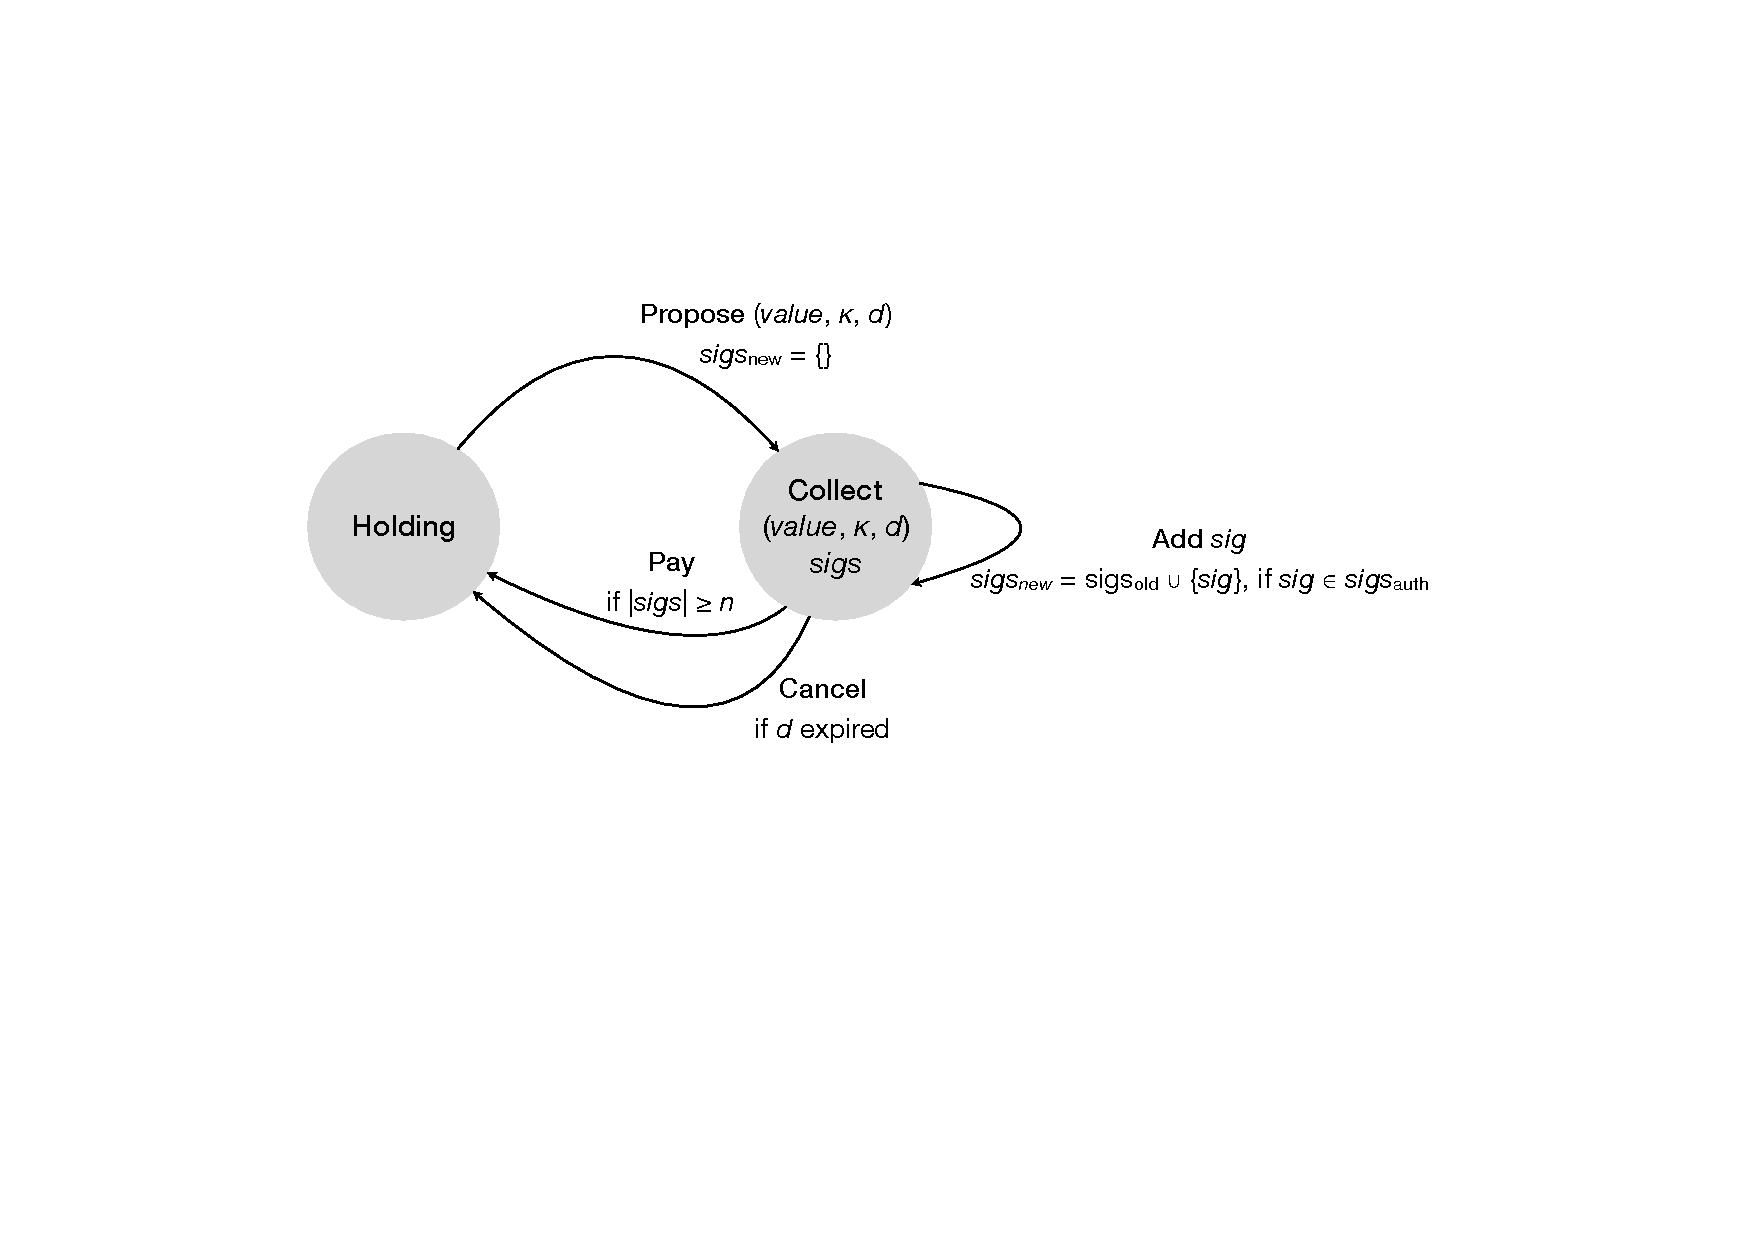
\includegraphics[width=\textwidth]{EUTxO_MultiSig_States.pdf}
  \caption{Transition diagram for the multi-signature state machine; edges labelled with input from redeemer and transition constraints.}
  \label{fig:multisig-machine}
\end{figure}
%
As a simple example of a state machine contract consider an $n$ out of $m$ multi-signature contract. Specifically, we have a given amount $\val_\msc$ of some cryptocurrency and we require the approval of at least $n$ out of an a priori fixed set of $m >= n$ owners to spend $\val_\msc$. With plain \UTXO{} (e.g., on Bitcoin), a multi-signature scheme requires out-of-band (off-chain) communication to collect all $n$ signatures to spend $\val_\msc$. On Ethereum, and also in the \EUTXO{} model, we can collect the signatures on-chain, without any out-of-band communication. To do so, we use a state machine operating according to the transition diagram in Figure~\ref{fig:multisig-machine}, where we assume that the threshold $n$ and authorised signatures $\sigs_\auth$ with \(|\sigs_\auth| = m\) are baked into the contract code.

In its implementation in the \EUTXO{} model, we use a validator function $\nu_\msc$ accompanied by the data value $\rho_\msc$ to lock $\val_\msc$. The data value $\rho_\msc$ stores the machine state, which is of the form \(\Holding\) when only holding the locked value or \(\Collecting{(\val, \kappa, d)}{\sigs}\) when collecting signatures $\sigs$ for a payment of $\val$ to $\kappa$ by the deadline $d$. The initial output for the contract is \((\nu_\msc, \val_\msc, \Holding)\).

The validator $\nu_\msc$ implements the state transition diagram from
Figure~\ref{fig:multisig-machine} by using the redeemer of the spending input to determine the transition that needs to be taken. That redeemer (state machine input) can take four forms: 
\begin{inparaenum}[(1)]
\item \(\Propose{\val, \kappa, d}\) to propose a payment of $\val$ to $\kappa$
  by the deadline $d$, 
\item \(\Add{\sig}\) to add a signature $\sig$ to a payment, 
\item $\Cancel$ to cancel a proposal after its deadline expired, and 
\item $\Pay$ to make a payment once all required signatures have been collected. 
\end{inparaenum}
It then validates that the spending transaction $\mi{tx}$ is a valid representation of the newly reached machine state. This implies that $\mi{tx}$ needs to keep $\val_\msc$ locked by $\nu_\msc$ and that the state in the data value $\rho'_\msc$ needs to be the successor state of $\rho_\msc$ according to the transition diagram.

The increased expressiveness of the \EUTXO{} model goes far beyond simple contracts such as this on-chain multi-signature contract. For example, the complete functionality of the Marlowe domain-specific language for financial contracts~\cite{marlowe} has been successfully implemented as a state machine on the \EUTXO{} model.

\section{Formal model}
\label{sec:formal-model}

\subsection{Basic types and notation}
\label{sec:basic-notation}
Figure~\ref{fig:basic-types} defines some basic types and
notation used in the rest of the paper; we have generally followed the
notation established by Zahnentferner in~\cite{Zahnentferner18-UTxO}.

\begin{ruledfigure}{!ht}
  \begin{displaymath}
    \begin{array}{rll}
      \B{} && \mbox{the type of booleans}\\
      \N{} && \mbox {the type of natural numbers}\\
      \Z{} && \mbox {the type of integers}\\
      (\phi_1 : T_1, \ldots, \phi_n : T_n) && \mbox{a record type with fields $\phi_1, \ldots, \phi_n$ of types $T_1, \ldots, T_n$}\\
      t.\phi && \mbox{the value of $\phi$ for $t$, where $t$ has type $T$ and
                $\phi$ is a field of $T$}\\
      \Set{T} && \mbox{the type of (finite) sets over $T$}\\
      \List{T} && \mbox{the type of lists over $T$, with $\_[\_]$ as indexing
        and $|\_|$ as length}\\
      h::t && \mbox{the list with head $h$ and tail $t$}\\
      x \mapsto f(x) && \mbox{an anonymous function}\\
      \hash{c} && \mbox{a cryptographic collision-resistant hash of $c$}\\
      \Interval{A} && \mbox{the type of intervals over a totally-ordered set $A$}
    \end{array}
  \end{displaymath}
  \caption{Basic types and notation}
  \label{fig:basic-types}
\end{ruledfigure}

\subsubsection{The \Data{} type.}
\label{sec:data}
We will make particular use of a primitive type \Data{} which can be
used to pass information into scripts. This is intended to be any
relatively standard structured data format, for example JSON or
CBOR~\cite{cbor}.

The specific choice of type does not matter for this paper, so we have left it
abstract. The intention is that this should
be well supported by all the programming languages we are interested in,
including whatever language is used for scripts, and whatever languages
are used for off-chain code that interacts with the chain.

We assume that for every (non-function) type $T$ in the scripting
language we have corresponding \toData{} and \fromData{} functions.

\subsection{\EUTXO{}: Enhanced scripting}
\label{sec:eutxo}
Our first change to the standard UTXO model is that as well as the
validator we allow transaction outputs to carry a piece of data called
the \emph{datum} (or \emph{datum object}), which is passed in as an
additional argument during validation.  This allows a contract to
carry some state (the datum) without changing its ``code'' (the
validator). We will use this to carry the state of our state machines
(see Section~\ref{sec:informal-eutxo}).

The second change is that the validator receives some information
about the transaction that is being validated. This information, which
we call the \textit{context}, is passed in as an additional
argument of type \ctx{}. The information supplied in the 
context enables the validator to enforce much stronger conditions than
is possible with a bare \UTXO{} model --- in particular, it can
inspect the \emph{outputs} of the current transaction, which is
essential for ensuring contract continuity (see
Section~\ref{sec:informal-eutxo}).

The third change is that we provide some access to time by adding a
\emph{validity interval} to transactions.
This is an interval of ticks (see Subsection~\ref{para:ticks})
during which a transaction can be processed (a generalisation of a ``time-to-live'').
Thus, any scripts which run during validation can assume that the current tick
is within that interval, but do not know the precise value of the current tick.

Finally, we represent all the arguments to the validator (redeemer, datum,
\ctx) as values of type \Data{}. Clients are therefore responsible for encoding
whatever types they would like to use into \Data{} (and decoding them inside the
validator script).

\subsection{A Formal Description of the \EUTXO{} Model}
\label{section:eutxo-spec}

In this section we give a formal description of the \EUTXO{} model.  The
description is given in a straightforward set-theoretic form, which
\begin{inparaenum}[(1)]
\item admits an almost direct translation into languages like Haskell for implementation, and
\item is easily amenable to mechanical formalisation.
\end{inparaenum}
We will make use of this in Section~\ref{sec:expressiveness}.

The definitions in this section are essentially the definitions of
\UTXO{}-based cryptocurrencies with scripts from
Zahnentferner~\cite{Zahnentferner18-UTxO}, except that we have made the changes
described above.

Figure~\ref{fig:eutxo-types} lists the types and operations used in the
the basic \EUTXO{} model. Some of these are defined here, the others must be provided by
the ledger (``ledger primitives'').
%%
\begin{ruledfigure}{!ht}
  \begin{displaymath}
  \begin{array}{rll}
    \multicolumn{3}{l}{\textsc{Ledger primitives}}\\
    \qty{} && \mbox{an amount of currency}\\
    \tick && \mbox{a tick}\\
    \Address && \mbox{an ``address'' in the blockchain}\\
    \Data && \mbox{a type of structured data}\\
    \DataHash && \mbox{the hash of a value of type \Data{}}\\
    \TxId && \mbox{the identifier of a transaction}\\
    \txId : \eutxotx \rightarrow \TxId && \mbox{a function computing the identifier of a transaction}\\
    \script && \mbox{the (opaque) type of scripts}\\
    \scriptAddr : \script \rightarrow \Address && \mbox{the address of a script}\\
    \hashData : \Data \rightarrow \DataHash && \mbox{the hash of an object of type\Data}\\
    \llbracket \_ \rrbracket : \script \rightarrow \Data \times \Data \times
    \Data \rightarrow \B && \mbox{applying a script to its arguments}\\
    \\
    \multicolumn{3}{l}{\textsc{Defined types}}\\
    \s{Output } &=&(\val: \qty,\\
                & &\ \addr: \Address,\\
                & &\ \datumHsh: \DataHash)\\
    \\
    \s{OutputRef } &=&(\txrefid: \TxId, \idx: \N)\\
    \\
    \s{Input } &=&(\outputref: \s{OutputRef},\\
               & &\ \validator: \script,\\
               & &\ \datum: \Data,\\
               & &\ \redeemer: \Data)\\
     \\
     \eutxotx\s{ } &=&(\inputs: \Set{\s{Input}},\\
                   & &\ \outputs: \List{\s{Output}},\\
                   & &\ \validityInterval: \Interval{\tick})\\
     \\
     \s{Ledger } &=&\!\List{\eutxotx}\\
  \end{array}
  \end{displaymath}
  \caption{Primitives and types for the \EUTXO{} model}
  \label{fig:eutxo-types}
\end{ruledfigure}

\paragraph{Addresses.}
We follow Bitcoin in referring to the targets of transaction outputs as
``addresses''. In this system, they refer only to \emph{script} addresses
(likely a hash of the script), but in a full system they would likely include
public-key addresses, and so on.

\paragraph{Ticks.}
\label{para:ticks}
A tick is a monotonically increasing unit of progress in the
ledger system. This corresponds to the ``block number''
or ``block height'' in most blockchain systems. We assume that there is some
notion of a ``current tick'' for a given ledger.

\paragraph{Inputs and outputs.} Transactions have a
\textsf{Set} of inputs but a \textsf{List} of outputs. There
are two reasons that we do not also have a \textsf{Set} of outputs although they
are conceptually symmetrical:
\begin{itemize}
\item We need a way to uniquely identify a transaction output, so
  that it can be referred to by a transaction input that spends it. The pair of
  a transaction id and an output index is sufficient for this, but other schemes
  are conceivable.
\item A \textsf{Set} requires a notion of equality. If we use the
  obvious structural equality on outputs, then if we had two outputs
  paying $X$ to address $A$, they would be equal. We need to
  distinguish these --- outputs must have an identity beyond
  just their address and value.
\end{itemize}

\paragraph{The location of validators and datum objects.} Validator scripts
and full datum objects are provided as parts of transaction \emph{inputs},
even though they are conceptually part of the output being spent. The
output instead specifies them by providing the corresponding address
or hash.\footnote{That these match up is enforced by
  Rules~\ref{rule:validator-scripts-hash} and
  \ref{rule:datums-hash} in Figure~\ref{fig:eutxo-validity}.}

This strategy reduces memory requirements, since
the \UTXO{} set must be kept in memory for rapid access while validating
transactions. Hence it is desirable to keep outputs small --- in
our system they are constant size.
Providing the much larger validator script only at the point where it is needed
is thus a helpful saving. The same considerations apply to datum objects.

An important question is how the person who spends an output \emph{knows} which
validator and datum to provide in order to match the hashes on the output.
This can always be accomplished via some off-chain mechanism, but we may
want to include some on-chain way of accomplishing this.\footnote{\Cardano{} will provide
a mechanism in this vein.} However, this is not directly relevant to this paper,
so we have omitted it.

\paragraph{Fees, forge, and additional metadata.}  Transactions will typically
have additional metadata, such as transaction fees or a ``forge''
field that allows value to be created or destroyed. These are
irrelevant to this paper, so have been omitted.\footnote{ Adding such
  fields might require amending Rule~\ref{rule:value-is-preserved}
  below to ensure value preservation.  }

\paragraph{Ledger structure.} We model a ledger as a simple
list of transactions: a real blockchain ledger will be more complex
than this, but the only property that we really require is that
transactions in the ledger have some kind of address which allows them
to be uniquely identified and retrieved.

\subsection{The \ctx{} type}
\label{sec:validation-context}
Recall from the introduction to Section~\ref{sec:eutxo} that when a
transaction input is being validated, the validator script is supplied
with an object of type \ctx{} (encoded as \Data{}) which contains
information about the current transaction.  The \ctx{} type is defined
in Figure~\ref{fig:ptx-1-types}, along with some related types.

\begin{ruledfigure}{!ht}
  \begin{displaymath}
  \begin{array}{rll}
    \s{OutputInfo } &=&(\val: \qty,\\
                    & &\ \i{validatorHash}: \Address,\\
                    & &\ \datumHsh: \DataHash)\\
    \\
    \s{InputInfo } &=&(\outputref: \s{OutputRef},\\
                   & &\ \i{validatorHash}: \Address,\\
                   & &\ \i{datum}: \Data,\\
                   & &\ \i{redeemer}: \Data,\\
                   & &\ \val: \qty)\\
     \\
     \ctx\s{ } &=&(\i{inputInfo}: \Set{\s{InputInfo}},\\
               & &\ \i{outputInfo}: \List{\s{OutputInfo}},\\
               & &\ \i{validityInterval}: \Interval{\tick},\\
               & &\ \i{thisInput}: \N)\\
     \\
  \end{array}
  \end{displaymath}
  \caption{The \ctx{} type for the \EUTXO{} model}
  \label{fig:ptx-1-types}
\end{ruledfigure}

\paragraph{The contents of \ctx{}.}
The \ctx{} type is a summary of the information contained in the $\eutxotx$ type in
Figure~\ref{fig:eutxo-types}, situated in the context of a validating
transaction, and made suitable for consumption in a script. That results in the following changes:
\begin{enumerate}
\item The \s{InputInfo} type is augmented with information that comes
  from the output being spent, specifically the value attached to that output.
\item The \ctx{} type includes an index that indicates the input currently
  being validated. This allows scripts to identify their own address, for example.
\item Validators are included as their addresses, rather than as scripts. This
  allows easy equality comparisons without requiring script languages to be able
  to represent their own programs.
\end{enumerate}
\noindent We assume that there is a function $\toCtx: \eutxotx \times
  \s{Input} \times \s{Ledger} \rightarrow \ctx$ which summarises a
transaction in the context of an input and a ledger state.
%% kwxm: moved this out of the figure because adding the Ledger
%% parameter pushed everything too far to the right.

\paragraph{Determinism.}
The information provided by \ctx{} is entirely determined by the
transaction itself. This means that script execution during validation
is entirely deterministic, and can be simulated accurately by the user
\emph{before} submitting a transaction: thus both the outcome of
script execution and the amount of resources consumed can be
determined ahead of time. This is helpful for systems that charge for
script execution, since users can reliably compute how much they will
need to pay ahead of time.

A common way for systems to violate this property is by providing
access to some piece of mutable information, such as the current time
(in our system, the current tick has this role). Scripts can then
branch on this information, leading to non-deterministic behaviour. We
sidestep this issue with the validation interval mechanism (see the
introduction to Section~\ref{sec:eutxo}).

\begin{ruledfigure}{!ht}
  \begin{displaymath}
  \begin{array}{lll}
  \multicolumn{3}{l}{\lookupTx : \s{Ledger} \times \TxId \rightarrow \eutxotx{}}\\
  \lookupTx(l,id) &=& \textrm{the unique transaction in $l$ whose id is $id$}\\
  \\
  \multicolumn{3}{l}{\txunspent : \eutxotx \rightarrow \Set{\s{OutputRef}}}\\
  \txunspent(t) &=& \{(\txId(t),1), \ldots, (\txId(id),\left|t.outputs\right|)\}\\
  \\
  \multicolumn{3}{l}{\unspent : \s{Ledger} \rightarrow \Set{\s{OutputRef}}}\\
  \unspent([]) &=& \emptymap \\
  \unspent(t::l) &=& (\unspent(l) \setminus t.\inputs) \cup \txunspent(t)\\
  \\
  \multicolumn{3}{l}{\getSpent : \s{Input} \times \s{Ledger} \rightarrow \s{Output}}\\
  \getSpent(i,l) &=& \lookupTx(l, i.\outputref.\id).\outputs[i.\outputref.\idx]
  \end{array}
  \end{displaymath}
  \caption{Auxiliary functions for \EUTXO{} validation}
  \label{fig:validation-functions-1}
\end{ruledfigure}


\subsection{Validity of \EUTXO{} transactions}
\label{sec:eutxo-validity}

Figure~\ref{fig:eutxo-validity} defines what it means for a transaction $t$
to be valid for a ledger $l$ during the tick \currentTick, using some auxiliary functions from
Figure~\ref{fig:validation-functions-1}.
Our definition combines
Definitions 6 and 14 from Zahnentferner~\cite{Zahnentferner18-UTxO}, differing from
the latter in Rule~\ref{rule:all-inputs-validate}.

This definition extends to an entire ledger: a ledger
$l$ is \textit{valid} if either $l$ is empty or
$l$ is of the form $t::l^{\prime}$ with
$l^{\prime}$ valid and $t$ valid for $l^{\prime}$.
%%
\vspace{-2mm}
%%
\begin{ruledfigure}{H}
\begin{enumerate}

\item
  \label{rule:tick-in-range}
  \textbf{The current tick is within the validity interval}
  \begin{displaymath}
    \currentTick \in t.\validityInterval
  \end{displaymath}

\item
  \label{rule:all-outputs-are-non-negative}
  \textbf{All outputs have non-negative values}
  \begin{displaymath}
    \textrm{For all } o \in t.\outputs,\ o.\val \geq 0
  \end{displaymath}

\item
  \label{rule:all-inputs-refer-to-unspent-outputs}
  \textbf{All inputs refer to unspent outputs}
  \begin{displaymath}
    \{i.\outputref : i \in t.\inputs \} \subseteq \unspent(l).
  \end{displaymath}

\item
  \label{rule:value-is-preserved}
  \textbf{Value is preserved}
  \begin{displaymath}
    \textrm{Unless $l$ is empty, } \sum_{i \in t.\inputs} \getSpent(i, l).\val = \sum_{o \in t.\outputs} o.\val
  \end{displaymath}

\item
  \label{rule:no-double-spending}
  \textbf{No output is double spent}
  \begin{displaymath}
    \textrm{If } i_1, i_2 \in t.\inputs \textrm{ and }  i_1.\outputref = i_2.\outputref
    \textrm{ then } i_1 = i_2.
  \end{displaymath}

\item
  \label{rule:all-inputs-validate}
  \textbf{All inputs validate}
  \begin{displaymath}
    \textrm{For all } i \in t.\inputs,\ \llbracket
    i.\validator\rrbracket (i.\datum,\, i.\redeemer,\,  \toData(\toCtx(t,i,l))) = \true.
  \end{displaymath}

\item
  \label{rule:validator-scripts-hash}
  \textbf{Validator scripts match output addresses}
  \begin{displaymath}
    \textrm{For all } i \in t.\inputs,\ \scriptAddr(i.\validator) = \getSpent(i, l).\addr
  \end{displaymath}

\item
  \label{rule:datums-hash}
  \textbf{Each datum matches its output hash}
  \begin{displaymath}
    \textrm{For all } i \in t.\inputs,\ \hashData(i.\datum) = \getSpent(i, l).\datumHsh
  \end{displaymath}

\end{enumerate}
\caption{Validity of a transaction $t$ in the \EUTXO{} model}
\label{fig:eutxo-validity}
\end{ruledfigure}
%%
%% kwxm: some dubious fiddling with vertical space to get the validity
%% figure in the right place and still stay within the page limit
%%
\vspace{-8mm}
\paragraph{Creating value.}
Most blockchain systems have special rules for creating or destroying value.
These are usually fairly idiosyncratic, and are not relevant to this paper, so
we have provided a simple genesis condition in
Rule~\ref{rule:value-is-preserved} which allows the initial transaction in the ledger
to create value.
\vspace{-1mm}
\paragraph{Lookup failures.}
The function $\getSpent$ calls $\lookupTx$, which looks up the unique
transaction in the ledger with a particular id and can of course
fail. However Rule~\ref{rule:all-inputs-refer-to-unspent-outputs}
ensures that during validation all of the transaction inputs refer to
existing unspent outputs, and in these circumstances $\lookupTx$ will
always succeed for the transactions of interest.


\section{Expressiveness of \EUTXO{}}
\label{sec:expressiveness}

In this section, we introduce a class of state machines that can admit
a straightforward modelling of smart contracts running on an \EUTXO{}
ledger. The class we choose corresponds closely to Mealy
machines~\cite{mealy} (deterministic state transducers). The transition
function in a Mealy machine produces a value as well as a new
state. We use this value to model the emission of constraints which
apply to the current transaction in the ledger. We do not claim that
this class captures the full power of the ledger: instead we choose it
for its simplicity, which is sufficient to capture a wide variety of
use cases.

We demonstrate how one can represent a smart contracts using Mealy
machines and formalise a \textit{weak bisimulation} between the
machine model and the ledger model.  Furthermore, we have mechanised
our results in Agda\site{
https://github.com/\GitUser/formal-utxo/tree/\AgdaCommit/Bisimulation.agda
}, based on an executable
specification of the model described in
Section~\ref{sec:formal-model}.

\subsection{Constraint Emitting Machines}
We introduce Constraint Emitting Machines (\CEM{}) which are based on
Mealy machines. A \CEM{} consists of its type of states \s{S} and inputs
\s{I}, a predicate function $\s{final} : \s{S} \rightarrow \s{Bool}$
indicating which states are final and a valid set of transitions,
given as a function $\s{step} : \s{S} \rightarrow \s{I} \rightarrow
\s{Maybe}\ (\s{S} \times \s{TxConstraints})$\footnote{
The result may be \s{Nothing}, in case no valid transitions exist from a given state/input.
}
from source state and input symbol to target state and constraints and
denoted $\CStep{s}{i}{\txeq}$.

The class of state machines we are concerned with here diverge from
the typical textbook description of Mealy Machines in the following aspects:
\begin{itemize}
\item The set of states can be infinite.

\item There is no notion of \textbf{initial state}, since we would not
  be able to enforce it on the blockchain level. Therefore, each
  contract should first establish some initial trust to bootstrap the
  process.
  One possible avenue for overcoming this limitation is to built a notion of \textit{trace simulation}
  on top of the current relation between single states,
  thus guaranteeing that only valid sequences starting from initial states appear on the ledger.
  For instance, this could be used to establish inductive properties of a state machine and
  carry them over to the ledger; we plan to investigate such concerns in future work.

\item While \textbf{final states} traditionally indicate that the
  machine \textit{may} halt at a given point, allowing this
  possibility would cause potentially stale states to clutter the \UTXO{}
  set in the ledger. Thus, a \CEM{} final state indicates that the
  machine \textit{must} halt. It will have no continuing transitions
  from this point onward and the final state will not appear in the
  \UTXO{} set. This corresponds to the notion of a \emph{stopped}
  process~\cite{sangiorgi} which cannot make any transitions.

\item The set of output values is fixed to \emph{constraints} which
  impose a certain structure on the transaction that will implement
  the transition.  Our current formalisation considers a limited set
  of first-order constraints, but these can easily be extended without
  too many changes in the accompanying proofs.
\end{itemize}

\subsection{Transitions-as-transactions}

We want to compile a smart contract $\mathcal{C}$ defined as a \CEM{} into
a smart contract that runs on the chain. The idea is to derive a
validator script from the step function, using the data value to hold the
state of the machine, and the redeemer to provide the transition signal.
A valid transition in a \CEM{}
will correspond to a single valid transaction on the chain. The
validator is used to determine whether a transition is valid and the
state machine can advance to the next state. More specifically, this
validator should ensure that we are transitioning to a valid target
state, the corresponding transaction satisfies the emitted constraints
and that there are no outputs in case the target state is final:

\[
\mkValidator{\mathcal{C}}(s, i, \mi{txInfo}) = \left\{
  \begin{array}{lll}
  \true  & \mi{if} \ \CStep{s}{i}{\txeq} \\
         & \mi{and} \ \satisfies(\mi{txInfo}, \txeq) \\
         & \mi{and} \ \checkOutputs(s', \mi{txInfo}) \\
  \false & \mi{otherwise}
  \end{array}
\right.
\]

\noindent
Note that unlike the step function which returns the new state, the
validator only returns a boolean. On the chain the next state is
provided with the transaction output that ``continues'' the state
machine (if it continues), and the validator simply validates that
the correct next state was provided.\footnote{
A user can run the step function locally to determine the correct next state off-chain.
}

\subsection{Behavioural Equivalence}
We have explained how to compile state machines to smart contracts but
how do we convince ourselves that these smart contracts will behave as
intended? We would like to show
\begin{inparaenum}[(1)]
\item that any valid transition in a \CEM{} corresponds to a valid transaction
  on the chain, and
\item that any valid transaction on the chain corresponds to a valid transition.
\end{inparaenum}
We refer to these two properties as soundness and completeness below.

While state machines correspond to automata, the automata theoretic
notion of equivalence --- trace equivalence --- is too coarse when we
consider state machines as running processes. Instead we use
bisimulation which was developed in concurrency theory for exactly
this purpose, to capture when processes behave the
same~\cite{sangiorgi}. We consider both the state machine and the
ledger itself to be running processes.

If the state machine was the only user of the ledger then we could
consider so-called strong bisimulation where we expect transitions in
one process to correspond to transitions in the other and
vice-versa. But, as we expect there to be other unrelated transactions
occurring on the ledger we instead consider weak bisimulation where
the ledger is allowed to make additional so-called \emph{internal}
transitions that are unrelated to the behaviour we are interested in
observing.

The bisimulation proof relates steps of the \CEM{} to new transaction
submissions on the blockchain.  Note that we have a \textit{weak}
bisimulation, since it may be the case that a ledger step does not
correspond to a \CEM{} step.

\begin{definition}[Process relation]
A \CEM{} state $s$ corresponds to a ledger $l$ whenever $s$ appears
in the current \UTXO{} set,
locked by the validator derived from this \CEM{}:
\[
\Sim{l}{s}
\]
\end{definition}

\begin{definition}[Ledger step]
Concerning the blockchain transactions, we only consider valid
ledgers.\footnote{ In our formal development, we enforce validity
  statically at compile time.  }  Therefore, a valid step in the
ledger consists of submitting a new transaction $tx$,
valid w.r.t. to the current ledger $l$,
resulting in an extended ledger $l'$:
\[
\LStep{l}{tx}
\]
\end{definition}

\begin{proposition}[Soundness]
Given a valid \CEM{} transition $\CStep{s}{i}{\txeq}$ and a valid ledger
$l$ corresponding to source state $s$, we can construct a valid
transaction submission to get a new, extended ledger $l'$ that
corresponds to target state $s'$:
\[
\infer[\textsc{sound}]
  {\exists tx\ l'\ .\ \LStep{l}{tx}\ \wedge \Sim{l'}{s'}}
  {%
    \CStep{s}{i}{\txeq}
  & \Sim{l}{s}
  }
\]
\end{proposition}

\paragraph{Note.}
We also require that the omitted constraints are satisfiable in the
current ledger and the target state is not a final one, since there
would be no corresponding output in the ledger to witness
$\Sim{l'}{s'}$.  We could instead augment the definition of
correspondence to account for final states, but we refrained from
doing so for the sake of simplicity.

\begin{proposition}[Completeness]
Given a valid ledger transition $\LStep{l}{tx}$ and a \CEM{} state $s$
that corresponds to $l$, either $tx$ is irrelevant to the current \CEM{}
and we show that the extended ledger $l'$ still corresponds to source
state $s$, or $tx$ is relevant and we exhibit the corresponding \CEM{}
transition $\CStep{s}{i}{\txeq}$\footnote{ We cannot provide a
  correspondence proof in case the target state is final, as explained
  in the previous note.  }:
\[
\infer[\textsc{complete}]
  { \Sim{l'}{s}\ \vee\ \exists i\ s'\ \txeq\ .\ \CStep{s}{i}{\txeq} }
  { \LStep{l}{tx}
  & \Sim{l}{s}
  }
\]
\end{proposition}

Together, soundness and completeness finally give us weak bisimulation.
Note, however, that our notion of bisimulation differs from the textbook one (e.g. in Sangiorgi~\cite{sangiorgi}),
due to the additional hypotheses that concern our special treatment of constraints and final states.

\section{Related work}
\label{sec:related}

Bitcoin Covenants~\cite{moser2016bitcoin} allow Bitcoin transactions to
restrict how the transferred value can be used in the future, including propagating
themselves to ongoing outputs. This provides contract continuity and allows the
implementation of simple state machines. Our work is inspired by Covenants, although
our addition of a data value is novel and simplifies the state passing.

The Bitcoin Modelling Language (BitML)~\cite{bitml} is an idealistic process calculus
that specifically targets smart contracts running on Bitcoin.
The semantics of BitML contracts essentially comprise a (labelled) \textit{transition system}, aka a state machine.
Nonetheless, due to the constrained nature of the plain \UTXO{} model without any extensions,
the construction is far from straightforward and requires quite a bit of off-chain communication to set everything up.
Most importantly, the BitML compilation scheme only concerns a restricted form of state machines,
while ours deals with a more generic form that admits any user-defined type of states and inputs.
BitML builds upon an abstract model of Bitcoin transactions by the same
authors~\cite{formal-model-of-bitcoin-transactions};
one of our main contributions is an extended version of such an abstract model,
which also accounts for the added functionality apparent in \Cardano{}.

Ethereum and its smart contract language, Solidity~\cite{Solidity} are powerful
enough to implement state machines, due to their native support for
global contract instances and state. However, this approach has some major downsides,
notably that contract state is global, and must be kept indefinitely by all core nodes.
In the \EUTXO{} model, contract state is localised to where it is used, and
it is the responsibility of clients to manage it.

Scilla~\cite{scilla} is a intermediate-level language for writing smart
contracts as state machines. It compiles to Solidity and is amendable to formal verification.
Since Scilla supports the asynchronous messaging capabilities of Ethereum,
Scilla contracts correspond to a richer class of automata, called
\textit{Communicating State Transition Systems}~\cite{csta}.
In the future, we plan to formally compare this class of state machines with our own class of \CEM{}s,
which would also pave the way to a systematic comparison of Ethereum's account-based model against \Cardano{}'s \UTXO{}-based one.

Finally, there has been an attempt to model Bitcoin contracts using \textit{timed automata}~\cite{timed-btc},
which enables semi-automatic verification using the UPPAAL model checker~\cite{uppaal}.
While this provides a pragmatic way to verify temporal properties of concrete smart contracts,
there is no formal claim that this class of automata actually corresponds to the semantics of Bitcoin smart contracts.
In contrast, our bisimulation proof achieves the bridging of this semantic gap.


\bibliographystyle{splncs04}
\bibliography{eutxo}

\end{document}
